\subsection{Giới thiệu}
\textbf{Scikit-learn} (viết tắt là \textbf{sklearn}) là một thư viện mã nguồn mở trong ngành machine learning, 
rất mạnh mẽ và thông dụng với cộng đồng Python, được thiết kế trên nền NumPy và SciPy. 
Scikit-learn chứa hầu hết các thuật toán machine learning hiện đại nhất, 
đi kèm với comprehensive documentations. Điểm mạnh của thư viện này là nó được sử dụng phổ biến trong giáo dục và công nghiệp, 
do đó nó luôn được cập nhật và có một cộng đồng người dùng đông đảo.
\begin{figure}[!htbp]
    \centering
    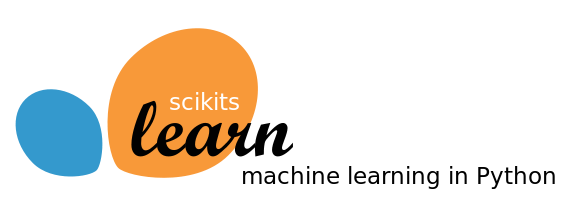
\includegraphics[scale=0.5]{scikit}
    \caption{Scikit}
    \label{fig:x cubed graph}
\end{figure}
\FloatBarrier
\subsection{Tại sao nên dùng Scikit?}
Hiện nay có nhiều thư viện mã nguồn mở phục vụ cho nghiên cứu machine learning. Bên cạnh Scikit-learn, có 2 thư viện nổi bật khác là
\begin{itemize}
    \item \textbf{LibSVM}: Được viết trên C bởi Chih-Chung Chang và Chih-Jen Lin. Như tên gọi của nó, thư viên này chứa các thuật toán SVM (Support Vector Machine), nhóm thuật toán mạnh mẽ hỗ trợ cả các tác vụ regression và classification.
    \item \textbf{TensorFlows}: Do các nhà khoa học của viện nghiên cứu Google Brain phát triển. TensorFlows được viết trên Python và là thư viện mở.
\end{itemize}
Trong khi TensorFlows có vẻ ở mức độ tiếp cận thấp hơn hơn thì Scikit-learn cho phép ta sử dụng ngay các thuật toán quan trọng một cách đơn giản và hiệu quả. 
Nói vậy không có nghĩa Scikit-learn là một thư viện “nông cạn”, Scikit-learn là nền tảng để xây dựng các ML implementations khác (Nilearn, Pylearn2,…). 
Scikit-learn còn là một trong những lựa chọn hàng đầu của các nhà nghiên cứu và phát triển. Đứng sau Scikit-learn là các viện nghiên cứu hàng đầu thế giới, gồm có Inria, Télécom Paristech, Paris-Saclay (Pháp), NYU Moore-Sloan Data Science Environment và Columbia University.